\documentclass[12pt]{report}
\usepackage[utf8]{inputenc}

\usepackage{adjustbox}
\usepackage{svg}
\usepackage{array}
\usepackage{multirow}
\usepackage{pdflscape}
\usepackage{afterpage}
\usepackage{longtable}
\usepackage{xcolor}

\usepackage{hyperref}
\usepackage{graphicx} % includegraphic 
\usepackage{placeins} % FloatBarrier 
\graphicspath{ {./figures/} }
\usepackage{mathptmx} % Font: Times
% ====== for styling Table of Content =====
\usepackage{tocloft}
% ====== for styling 'chapter' and 'section' ...
\usepackage{titlesec}
% ====== For math function =======
\usepackage{amsmath}
\usepackage{amssymb}
\let\mathcal\undefined
\DeclareMathAlphabet{\mathcal}{OMS}{cmsy}{m}{n}

% Chapter
\titleformat
{\chapter} % command
[display] % shape
{\bfseries\large\center} % format
{CHAPTER \thechapter} % label
{0.6em} % sep
{} % before-code
[] % after-code
% remove space above and set below 28pt space chapter
\titlespacing*{\chapter}{0pt}{-35pt}{28pt}

% Section (Heading, Level 2)
\titleformat
{\section} % command
[hang] % shape
{\bfseries} % format
{\thesection} % label
{0em} % sep
{ } % before-code
[] % after-code
% add 1.5 line space above section and remove line space after it
\titlespacing*{\section}{0pt}{1.6em}{0pt}

% subSection (Heading, Level 3)
\titleformat
{\subsection} % command
[hang] % shape
{\bfseries \itshape} % format
{\thesubsection} % label
{0em} % sep
{ } % before-code
[] % after-code
% add 0 line space above section and remove line space after it
\titlespacing*{\subsection}{0pt}{0em}{0pt}

% subsubSection (Heading, Level 4)
\titleformat
{\subsubsection} % command
[runin] % shape
{\bfseries} % format
{\thesubsubsection} % label
{0em} % sep
{ } % before-code
[] % after-code
% 0.5inch indent, 0 line space above, 1 space after header
\titlespacing*{\subsubsection}{0.5in}{0em}{1ex}

% ====== Indent ======
% By default, the first paragraph is not indent - we need this package for indentation
\usepackage{indentfirst}
% ====== list + enum ======
\usepackage{enumitem}
% Set indent lenght for itemize and enumerate
\setlist[itemize]{left=0.5in}
\setlist[enumerate]{left=0.5in}
% Remove separation between item
\setlist{nosep}
% ====== caption styling ======
\usepackage{caption}
\DeclareCaptionFormat{aitformat}{\textbf{#1} #2 \textit{#3}}
% justification = RaggedRight : Caption start on the left
% singlelinecheck = false     : Force caption to start on the left
% labelsep = newline          : separate Table 1.1 and label
\captionsetup{format = aitformat,
              justification = RaggedRight,
              singlelinecheck = false,
              labelsep = newline}
              
% ====== References ======
\usepackage[notocbib]{apacite}

% ====== Acronyms ======
\usepackage[acronym]{glossaries}
\newacronym{vl}{VL}{Vision language}
\newacronym{mlm}{MLM}{masked language modeling}
\newacronym{itc}{ITC}{image-text constrative learning}
\newacronym{itm}{ITM}{image-text matching}
\newacronym{vqa}{VQA}{visual question answering}
\newacronym{pos}{POS}{part of speech}
\newacronym{vgr}{VGR}{Visual Genome Relation}
\newacronym{vga}{VGA}{Visual Genome Attribution}
\newacronym{co}{Co}{COCO order}
\newacronym{fo}{Fo}{Filckr order}

% ====== Document begins here ======
\begin{document}
    % Set counter depth up to subsubsection (heading, level 4)
    \setcounter{secnumdepth}{3}
    
    % ====== include other section ======
    \addcontentsline{toc}{part}{TITLE PAGE}

\begin{titlepage}
%   everything on center
  \begin{center}
   
  \textbf{\large{ PART OF SPEECH EFFECT ON VISION-LANGUAGE REPRESENTATION LEARNING }}

  \vspace{3em} % (3 blank lines)
  
  by
  
  \vspace{3em} % (3 blank lines)
  
  Pasit Tiwawongrut
  
  \vspace{4em} % (4 blank lines)

  A Thesis Submitted in Partial Fulfillment of the Requirements for the Degree of Master of Science in Data Science and Artificial Intelligence

  \vspace{4em} % (4 blank lines)

\begin{center}
  \begin{tabular}{ rl }
Examination Committee: & Dr. Chaklam Silpasuwanchai (Chairperson)\\
                       & Dr. Chantri Polprasert \\
                       & Dr. Attaphongse Taparugssanagorn \\\\
                       
% UNCOMMENT THE LINES BELOW IF YOU HAVE THE EXTERNAL EXAMINER.
% External Examiner: & Prof. YOUR EXTERNAL EXAMINER  \\
%                   & Dept. of Electrical and Computer Engineering \\ 
%                   & McGill University, Canada \\ \\
\\ \\ \\
Nationality:     & Thai \\
Previous Degree: & Bachelor of Computer Engineering \\
                 & Khon Kaen University \\
                 & Thailand \\
\\
% *  For Self-Support – delete the line Scholarship Donor
Scholarship Donor: & Asian Institute of Technology
  \end{tabular}
\end{center}

\vspace{3em}

Asian Institute of Technology \\
School of Engineering and Technology \\
Thailand \\           
July 2025


  \end{center}
\end{titlepage}

    
    % Show page numbering as 'roman'
    \pagenumbering{roman}
    % Start page counter as 2
    \setcounter{page}{2}
    
    % add to Table of content
\addcontentsline{toc}{part}{ACKNOWLEDGMENTS}

% set 0 indentation
\setlength{\parindent}{0pt}
% set paragraph space = 1 space
\setlength{\parskip}{1em}
% set line space = 1
\setlength{\baselineskip}{1.5em} % this is the default value for line space = 1

\begin{center}
  \fontsize{14}{17}\selectfont{\textbf{
    ACKNOWLEDGMENTS
  }} \\
\end{center}
\vspace{36pt} 

Lorem ipsum dolor sit amet, consectetur adipiscing elit, sed do eiusmod tempor incididunt ut labore et dolore magna aliqua. Aliquam malesuada bibendum arcu vitae elementum. Aliquet enim tortor at auctor. Sodales ut eu sem integer vitae justo. Tellus pellentesque eu tincidunt tortor aliquam nulla facilisi. Ut lectus arcu bibendum at varius vel pharetra. Integer vitae justo eget magna. Mollis nunc sed id semper risus. Donec ac odio tempor orci dapibus ultrices in iaculis. Non arcu risus quis varius quam quisque id diam vel. Felis donec et odio pellentesque diam volutpat commodo sed egestas. Dignissim diam quis enim lobortis scelerisque. Placerat vestibulum lectus mauris ultrices eros in cursus.

%Ut venenatis tellus in metus vulputate eu scelerisque felis. Blandit volutpat maecenas volutpat blandit aliquam etiam erat velit. Ac felis donec et odio pellentesque diam volutpat commodo sed. Dignissim convallis aenean et tortor at risus viverra adipiscing at. Donec pretium vulputate sapien nec. Nisi porta lorem mollis aliquam. Sed nisi lacus sed viverra. Metus vulputate eu scelerisque felis imperdiet proin fermentum leo vel. Convallis convallis tellus id interdum velit laoreet id donec ultrices. Volutpat diam ut venenatis tellus in metus. Magna fringilla urna porttitor rhoncus dolor purus non enim. Eget mi proin sed libero enim sed faucibus turpis in. Bibendum ut tristique et egestas quis ipsum suspendisse. Tellus integer feugiat scelerisque varius morbi. Aliquet eget sit amet tellus. Massa tincidunt dui ut ornare lectus sit. Nunc scelerisque viverra mauris in aliquam sem fringilla. Cum sociis natoque penatibus et magnis dis parturient montes nascetur. Et egestas quis ipsum suspendisse ultrices. Mauris vitae ultricies leo integer malesuada nunc vel risus.
    % add to Table of content
\addcontentsline{toc}{part}{ABSTRACT}

% set 0 indentation
\setlength{\parindent}{0pt}
% set paragraph space = 1 space
\setlength{\parskip}{1em}
% set line space = 1.5
\setlength{\baselineskip}{1.5em}

\begin{center}
  \fontsize{14}{17}\selectfont{\textbf{
    ABSTRACT
  }}
\end{center}
\vspace{2em}

\acrfull{vl} models have shown promising performance across multiple tasks in both zero-shot and fine-tuning setups. 
Most studies use \acrlong{mlm} as a pre-training task, applying random masking to image caption tokens. 
However, random token masking is not an optimal strategy for training \acrshort{vl} models, and effective masking strategies in \acrshort{vl} remain underexplored. 
In this work, we investigate the effects of \acrfull{pos} masking, as each \acrshort{pos} category contributes differently to sentence meaning. 
By pre-training models with different \acrshort{pos} masking strategies, we evaluate each model on image-text retrieval and visual question answering tasks, categorizing each question type following the VALSE.
Our findings contribute to a deeper understanding of how \acrshort{pos} masking influences model performance, providing insights that can lead to more effective pre-training strategies for future \acrshort{vl} models.

% 4)  key findings (2-3 sentences)
%     - summarize ONLY the key findings - it means interesting findings
% 5)  contributions
%     - why this is important to be solved; what impact it can bring
    
% Exercise: within 15 mins, write down these five sentences, and then put on the chat.
% \textbf{Keywords:} keyword1, keyword2. 
    % Rename table of content to CONTENTS
\renewcommand\contentsname{\begin{center}
  \fontsize{14}{17}\selectfont{\bf{CONTENTS}}
\end{center}}
% set space above title
\renewcommand{\cftbeforetoctitleskip}{-35pt}
% set space below title
\renewcommand{\cftaftertoctitleskip}{0em}
% after title, skip 3 spaces and write 'page' on the right
\renewcommand{\cftaftertoctitle}{%
  \vspace{3em}
  \hfill{\textbf{Page}}
}
% Remove . from table of content
\renewcommand{\cftdot}{}

% styling part:
\renewcommand{\cftpartfont}{\fontsize{12}{14}\selectfont\bf} % set font bold for page name
\renewcommand{\cftpartpagefont}{\fontsize{12}{14}\selectfont\bf} % set font size and bold for page number
\setlength{\cftbeforepartskip}{0pt} % set line space

% styling chapter:
\renewcommand{\cftchapfont}{\bf{CHAPTER} \fontsize{12}{14}\selectfont\bf} % set font size bold, leading with 'CHAPTER'
\renewcommand{\cftchappagefont}{\fontsize{12}{14}\selectfont\bf} % set font size and bold for page number
\setlength{\cftbeforechapskip}{0pt} % set line space
\setlength{\cftsecindent}{4.5em}
\setlength{\cftsubsecindent}{7em}

% set dept of contents
\setcounter{tocdepth}{2}

% Print content
\tableofcontents
    \addcontentsline{toc}{part}{LIST OF TABLES}

% Rename List of Tables to CONTENTS
\renewcommand\listtablename{\begin{center}
  \fontsize{14}{17}\selectfont{LIST OF TABLES}
\end{center}}
% set space above title
\renewcommand{\cftbeforelottitleskip}{-25pt}
% set space below title
\renewcommand{\cftafterlottitleskip}{0em}
% after title, skip 3 spaces and write 'page' on the right
\renewcommand{\cftafterlottitle}{%
  \vspace{3em}
  \textbf{Tables}\hfill{\textbf{Page}}
}

% remove indent
\renewcommand{\cfttabindent}{0pt}
% add 'Table' before numbering
\renewcommand{\cfttabpresnum}{Table~}
% indent the table caption
\renewcommand{\cfttabnumwidth}{4.5em}

\begingroup
    \renewcommand*{\addvspace}[1]{}
    \listoftables
\endgroup
    \addcontentsline{toc}{part}{LIST OF FIGURES}

% Rename List of Tables to CONTENTS
\renewcommand\listfigurename{\begin{center}
  \fontsize{14}{17}\selectfont{LIST OF FIGURES}
\end{center}}
% set space above title
\renewcommand{\cftbeforeloftitleskip}{-25pt}
% set space below title
\renewcommand{\cftafterloftitleskip}{0em}
% after title, skip 3 spaces and write 'page' on the right
\renewcommand{\cftafterloftitle}{%
  \vspace{3em}
  \textbf{Figures}\hfill{\textbf{Page}}
}

% remove indent
\renewcommand{\cftfigindent}{0pt}
% add 'Table' before numbering
\renewcommand{\cftfigpresnum}{Figure~}
% indent the table caption
\renewcommand{\cftfignumwidth}{4.5em}

\begingroup
    \renewcommand*{\addvspace}[1]{}
    \listoffigures
\endgroup
    
    % Start page counter as 1
    \setcounter{page}{1}
    % Show page numbering as 'arabic'
    \pagenumbering{arabic}
    % set 0.5 inch indentation
\setlength{\parindent}{0in}
% set paragraph space = 0 space
\setlength{\parskip}{1.5mm}
% set line space 1.5
\setlength{\baselineskip}{1.6em}

\chapter{INTRODUCTION}
\section{Background}
Human describe real world by using a sentence, which compose of a strutural word with a specfic purpose, e.g noun refer to an entity, verb refer to an action, and adjective describe the detail of the entities.


\acrfull{vl} models have gained significant attention due to their ability to perform both zero-shot and transfer learning, achieving high performance across numerous downstream tasks through pre-training with web-scale image-text pairs \cite{s-clip, medclip, vl-review}.  
Many \acrshort{vl} models incorporated \acrfull{mlm} as a pre-training task, making it an important method to train \acrshort{vl} models \cite{albef, mplug, uniter, beit-3, lxmert}.  
Typically, a subset of word tokens is randomly masked at a percentage during training, and the model is tasked with predicting these masked tokens using information from both visual and language modalities.  
This masking approach has proven to enhance the alignment between visual and linguistic representations, boosting performance in \acrshort{vl} tasks \cite{lxmert}.  

Despite the widespread adoption of \acrshort{mlm} in \acrshort{vl} training, its effects on model performance, efficiency, and training loss remain underexplored.  
\citeA{mask_object} demonstrated that many of the randomly masked tokens are often stop-words or punctuation, which the model can easily learn without any need for masking.  
Another study by \citeA{selective_masking} demonstrated that selectively masking infrequent words from the pre-training dataset can boost model performance on out-of-domain datasets during continued training.  
Additionally, \citeA{rf-curriculum-masking} suggested that random masking causes the model to rely heavily on local text signals, and it results in inefficient and inconsistent interactions between modalities, leading to suboptimal performance.  
These findings emphasize the importance of strategic token selection in \acrshort{mlm} to enhance \acrshort{vl} model performance and efficiency.  

In this work, we aimed to address the gap in understanding how masking each \acrfull{pos} impacts \acrshort{vl} models.  
Each \acrshort{pos} contributes distinctively to sentence meaning: nouns typically denote objects, while verbs describe actions and often demand contextual comprehension.  
By selectively masking different parts of speech, we could better understand how each \acrshort{pos} category affects the alignment between visual and linguistic information.  
To further explore the effect of each \acrshort{pos}, training without the \acrshort{mlm} task and with different \acrshort{pos} masking ratios were compared.
The experiment is designed to answer the following questions:  
\begin{enumerate}  
    \item How does masking each \acrshort{pos} impact the performance, and training loss of \acrshort{vl} pre-training models?  
    \item How does each \acrshort{pos} masking strategy affect \acrfull{vqa} performance when analysed based on different question types?  
    \item What is the difference between training without the \acrshort{mlm} task compared to training with it, and when masking each \acrshort{pos} with a 100 percent masking ratio?  
\end{enumerate}


\section{Objective}  
The objectives for our experiment are as listed.  
\begin{enumerate}  
    \item Develop a pre-trained \acrshort{vl} model to evaluate the impact of masking each \acrshort{pos} on performance and training efficiency.  
    \item Benchmark the performance of each \acrshort{pos} masking approach using specialized datasets to gain a deeper understanding of masking effects with retrieval and question answering tasks.  
    \item Train the model without \acrshort{pos} masking and with \acrshort{pos} masking at a 100 percent masking ratio.  
\end{enumerate}  

\section{Scope}
\begin{enumerate}  
    \item The training and testing datasets are web-scale image-text pairs.  
    \item The model architecture is a cross-attention model, chosen for its ability to jointly predict answers based on information from multiple modalities, and training the model with \Acrshort{mlm} loss.
\end{enumerate}  

    \chapter{LITERATURE REVIEW}
This section of the literature review is organized around two key topics relevant to our study.
The first topic addresses \acrshort{vl} models, providing an overview of the model architectures recently used in \acrshort{vl} models and discussing the choice of the base architecture for the \acrshort{vl} model used in this research.
The second topic \acrshort{mlm}, an important pre-training approach that has improved \acrshort{vl} model performance.
Together, these sections provide a comprehensive overview of the methodological foundations of this study.

\section{Vision-Language model}
In the early stage of \acrshort{vl} learning, the goal of training is to align fine-grained features of the image with text. 
Many works have adopted object detection to create fine-grained labels for the training images \cite{uniter, vlmo}. 
However, the focus of \acrshort{vl} training has shifted to using web-scale image-text pairs as a training target, demonstrating competitive performance, as shown by CLIP \cite{clip}. 
\citeA{clip} proposed contrastive training for \acrshort{vl} with a large-scale image-text pairs dataset by optimizing the alignment of image and text encodings from the same pair, which was proven to be scalable by \citeA{align}. 
This approach has become a foundational model for \acrshort{vl} tasks \cite{foundation_model}.

Recent advancements in \acrshort{vl} model training can be roughly categorized into three main methods.  
The first approach is a separate unimodal encoder for each modality, as seen in models like CLIP \cite{clip} and ALIGN \cite{align}. 
This method is trained with the objective of aligning the intermediate outputs of each modality's encoding.  
The second method uses a cross-attention layer to fuse multimodal inputs, e.g., Flamingo \cite{flamingo}, mPLUG \cite{mplug}, LXMERT \cite{lxmert}, and ALBEF \cite{albef}. 
The cross-attention layer enables the model to fuse each modality more deeply.  
Finally, the third approach uses a single large attention model with concatenated image and text tokens as input, as in BEIT \cite{beit-3}. 
This approach allows for early-stage fusion of each modality, though it requires the highest amount of computational resources.  
In this work, we adopt the cross-attention method as the base model due to its effectiveness in fusing multimodal inputs. 
Additionally, this approach allows the model to be trained using the \acrshort{mlm} task.

\section{Masked Language Modelling}
\acrshort{mlm} is a widely used pre-training method in language model (LM) training \cite{bert, albert, dictbert, opt, realm} as a self-supervised task. 
BERT \cite{bert} proposed \acrshort{mlm} as a pre-training task, which has been proven effective for pre-training language models. 
The \acrshort{mlm} task involves replacing some input tokens with a special [MASK] token, and the model must predict the masked tokens based on the given unmasked tokens. 
In the field of \acrshort{vl} models, many \acrshort{vl} models have also adopted \acrshort{mlm} as a training task to train the model to predict masked text based on visual information \cite{albef, mplug, uniter, beit-3}.

In the field of selective masking strategies in natural language processing, several works have further refined \acrshort{mlm} to enhance training efficiency. 
ERNIE \cite{ERNIE}, SpanBERT \cite{spanBERT}, and \(n\)-gram Masking \cite{n-gram-masking} propose span masking instead of single-token masking, which forces the model to rely more on long-range dependencies rather than adjacent tokens, resulting in better performance compared to BERT \cite{bert}. 
Considering linguistic features, \citeA{posmaskinglearning} conducted a training analysis based on POS masking focused on LM training. 
The results showed that focusing the masking of non-function words (ADJ, ADV, NOUN, PROPN, and VERB) in the later stages of training can encourage the LM model to develop a better contextual understanding.

For selective masking in \acrshort{vl} training, \citeA{mask_object} introduced an object token masking strategy, selectively masking object tokens in image captions and pre-training the model. 
This approach achieved superior performance compared to random masking. 
Another study by \citeA{selective_masking} showed that selectively masking infrequent words from the pre-training dataset during continued training enhances model performance on out-of-domain datasets. 
Additionally, \cite{rf-curriculum-masking} proposed a curriculum-based masking strategy in which a reinforcement learning agent dynamically selects masking spans based on cross-modal interactions. 
This method improved the model’s mulitmodalities understanding while reducing the dataset size needed for effective training. 
In this work, we conduct experiments to analyze the impact of each \acrshort{pos} on results within a \acrshort{vl} setting.

% \section{Probing and interpretability}
% In order to analyze deep learning models, it is important to utilize both probing and interpretation methods. 
% We can divide model-agnostic methods into two categories: white-box methods, which leverage the internal structure and parameters of deep learning models to interpret the reasoning behind their outputs, and black-box methods, where we modify the input and observe the resulting changes in the model's output.

% For white-box methods, Grad-CAM \citeA{grad-cam} is a technique used with CNNs and Vision Transformers. 
% This method considers the gradient of the input to interpret the reasoning behind the model’s prediction. 
% \citeA{attention-explanations} proposed a method for interpreting attention scores. 
% However, these white-box methods are not well-suited for analyzing multimodal deep learning models to understand interactions between different modalities.

% For black-box methods, DIME \cite{dime} proposed an interpretation technique that probes a deep learning model using an interpretable linear function over the model’s output. 
% Another method to consider is Amnesic Probing \cite{amnesic-probing}, which uses causal intervention by removing parts of the input. 
% This allows us to measure the contribution of each part of the input to the model's output. 
% In the context of multimodal training, \citeA{mm-shap} proposed MM-Shap, inspired by Shapley values, to evaluate the contribution of each modality.

% In this work, we adopt MM-Shap as an interpretation method to analyze changes in the contribution of each modality.
% MM-Shap is specifically designed to handle multimodal inputs without considering the accuracy of a deep learning model. 
% It provides a quantitative measure of the contribution of each modality.
    \chapter{METHODOLOGY}
In this chapter, the methodology is detailed as follows. 
First, we describe the architecture of the model. 
Second, we explain the \acrshort{mlm} pre-training loss functions used in this experiment.
Third, the details of \acrshort{pos} tagging are provided. 
Fourth, we outline the datasets used in this experiment. 
Fifth, we provide details on the visual question answering setup.
Lastly, we provide implementation detail for the pre-training model.

\begin{figure}[h]
    \caption{Overall methodology}
    \label{fig:overview}
    Pre-training the model with a \acrshort{mlm} task by masking tokens based on the \acrshort{pos} in the image captions.
    \begin{center}
        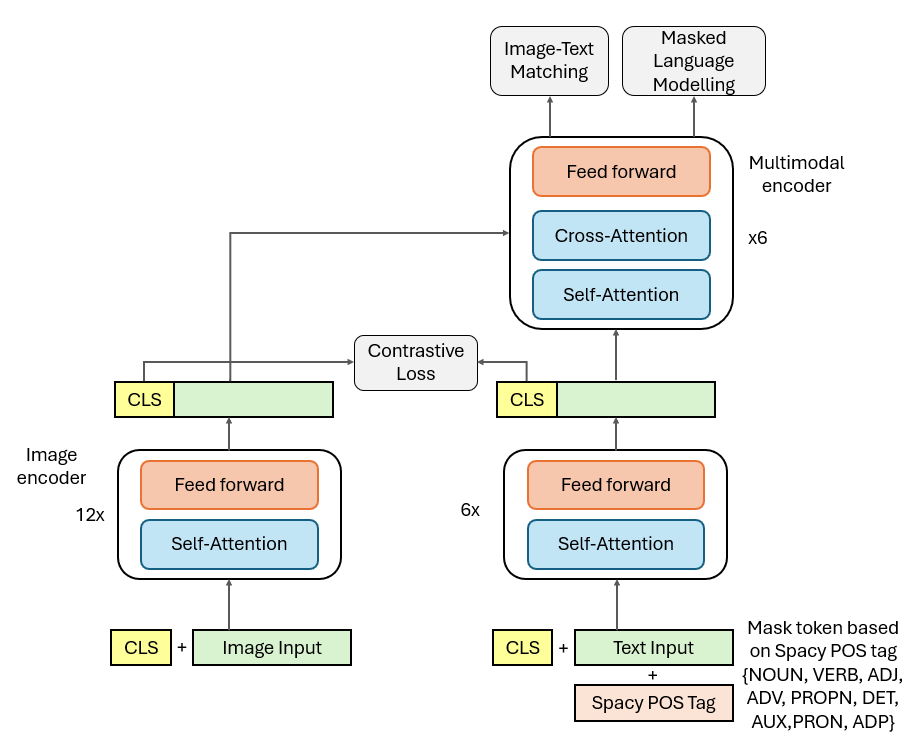
\includegraphics[width=0.8\textwidth]{Images/overview.png}
    \end{center}
    \small
\end{figure}

\section{Model architecture}
As shown in Figure \ref{fig:overview}, our model includes three main components: an image encoder, a text encoder, and a multimodal encoder. 
The first component is the image encoder, for which we use ViT \cite{vit}, modified following \cite{clip}, as the image encoder in this experiment. 
The second component is the text encoder, which employs a transformer architecture as BERT \cite{bert} to encode image captions.
The final component is the multimodal encoder, where \acrshort{vl} interactions occur.

Given a training dataset \(D\) consisting of image-text pairs \((I_i, T_i) \in D\), where \(I_i\) is the image and \(T_i\) is the image caption of the \(i\)-th image, each image is first encoded as a sequence of tokens \(\{v_{cls}, v_1, \dots, v_n\}\) using ViT \cite{vit}. 
Here, \(v_{cls}\) represents the embedding of the [CLS] token prepended to the image patch sequence. 
In this experiment, the image encoder was initialized with ViT-B-32 pre-trained on ImageNet-21K \cite{imagenet}.
Next, we use a 6-layer transformer, randomly initialized, to encode the image caption \(T_i\) into text embeddings \(\{w_{cls}, w_1, \dots, w_n\}\), where \(w_{cls}\) is the embedding of the [CLS] token. 
Finally, both text and image encodings are passed through the multimodal encoder to fuse both inputs, producing multimodal encodings. 
For the multimodal encoder, a cross-attention layer is used, where both keys and values are the image encodings, and the text encoding serves as the query in the cross-attention layer.


% Cross Attention using Image = K, V Text as a query.
% Thought: The image encoder choice can be change based on training speec.
\section{Pre-training objectives}
In this work, we pre-train our model with three objectives: \acrfull{mlm}, \acrfull{itc} and \acrfull{itm}.
\subsection{Mask language modelling}
Our model is trained with the \acrshort{mlm} task. 
Typically, a percentage of tokens \(\{w_1, \dots, w_T\}\) are replaced with a special [MASK] token to create a masked caption \(T^{\text{mask}}\). 
However, in this work, the masked tokens are selected based on \acrshort{pos} type instead of randomly masking. 
The model is then trained to predict the original tokens at the masked positions, conditioned on both the unmasked tokens in \(T^{\text{mask}}\) and the visual features of \(I\) as \(p^{\text{mask}}(I, T^{\text{mask}})\).
Let \(y^{\text{mask}}\) be a one-hot vector representing the ground-truth vocabulary for the masked token, where the masked token has a probability of 1. 
The model’s objective is to minimize the cross-entropy \(\mathbf{H}\), given by:
\[
    \mathcal{L}_{\text{MLM}} = \mathbf{H}(y^{\text{mask}}, p^{\text{mask}}(I, T^{\text{mask}})S))
\]

\subsection{Image-text contrative learning}
To improve each unimodal encoders representation, we use \acrshort{itc} to improve alignment of each modality.
\acrshort{itc} aims to improve alignment by maximize similarity score of image and text from the same pair with score function \(s(I, T) = v_{cls}^\top w_{cls}\), and minimize similarity score of image and text not from its pair.
We then calculate softmax-normalized similiarity score for each image to any text and each text to any image, identified as image-to-text \(p^{i2t} \in \mathbb{R}^{M}\) and text-to-image \(p^{t2i} \in \mathbb{R}^{M}\) score as:
\[
    p^{i2t}_i(I) = \frac{ \exp{(s(I,T_i))/\tau} }{ \sum_{m=1}^{M}\exp{(s(I,T_m)/\tau} }, \quad p^{t2i}_i(T) = \frac{ \exp{(s(T,I_i))/\tau} }{ \sum_{m=1}^{M}\exp{(s(T,I_m)/\tau} }
\]
where \(\tau\) is a learnable temperature parameter. Let \( y^{i2t}(I) \in \{0,1\}^M \) and \( y^{t2i}(T) \in \{0,1\}^M \) be a ground truth with probability of 1 at a position of same pair, and probability of 0 on the otherhand.
The \acrshort{itc} loss is calculated as cross-entropy \(\mathbf{H}\) between \(p\) and \(y\):
\[
    \mathcal{L}_{\text{ITC}} = \frac{1}{2}(\mathbf{H}(y^{i2t},p^{i2t}) + \mathbf{H}(y^{t2i},p^{t2i}))
\]
\subsection{Image-text matching}
\section{Part of speech tagging}


\section{Pre-training dataset}
We pre-trained the model on the Conceptual Captions dataset \cite{conceptual-caption}, which consists of 3.3 million image-text pairs. 
In Conceptual Captions dataset, an automated process was used to select, filter, and refine these image-caption pairs to ensure they are clear, informative, and suitable for effective model training.

\section{Evaluation}
In this work, we evaluate each model trained with different types of \acrshort{pos} masking using image-text retrieval and visual question answering tasks. 
The details of the evaluation methods and datasets are described in this section.


\subsection{Image-text retrieval}
For the image-text retrieval task, we evaluate the effect of masking on each \acrshort{pos} category by performing zero-shot evaluations on the Flickr30K \cite{flickr30k} and VALSE \cite{valse} datasets for both image-to-text and text-to-image retrieval. 
The Flickr30K dataset is used to assess the model's overall performance in retrieval tasks. 
For a deeper understanding, the VALSE dataset provides a breakdown of linguistic phenomena into six categories: existence, plurality, counting, relation, action, and coreference. 
Each image caption in the VALSE dataset also includes a "foil" version, in which words related to each caption category are altered. 
This approach enables us to analyze how different \acrshort{pos} masking strategies impact the model retrieval performance and the alignment between visual and textual representations.

\subsection{Visual question answering}
For visual question answering task, we assess each model with

% \section{Implementation Detail}
% BF16 datatype
    \chapter{Results}
In this chapter, we provide all the experiment results for each experiment and evaluation.

\section{Pre-training}

\subsection{Flickr30K}

\begin{table}[]
    \centering
    \label{tab:flickr30k}
    \caption{Flickr30K benchmark image retrieval result.}
    \begin{tabular}{ll|lll|lll}
        \multicolumn{2}{c|}{\multirow{3}{*}{Masking Method}} & \multicolumn{6}{c}{Flickr30K} \\
        \multicolumn{2}{l|}{} & \multicolumn{3}{l|}{\acrshort{tr}} & \multicolumn{3}{l}{\acrshort{ir}} \\
        \multicolumn{2}{l|}{} & r@1 & r@5 & r@10 & r@1 & r@5 & r@10 \\
        \hline
        \multicolumn{2}{c|}{Random Masking} & \cellcolor{yellow}67.00 & 88.00 & 93.75 & 52.61 & 80.14 & 87.76 \\
        \hline
        \multirow{5}{*}{Non-function} & Noun & 67.15 & 88.60 & 94.65 & 52.73 & 80.45 & 87.79 \\
        & Verb & 54.85 & 82.85 & 90.05 & 43.82 & 73.84 & 82.82 \\
        & Adj & 62.30 & 87.30 & 92.40 & 47.39 & 75.47 & 84.06 \\
        & Adv & 46.85 & 76.25 & 85.75 & 36.40 & 66.38 & 76.78 \\
        & PropN & 44.85 & 74.40 & 84.10 & 34.91 & 64.09 & 75.01 \\
        \hline
        \multirow{4}{*}{Function} & Det & 71.05 & 92.00 & 95.30 & 56.01 & 81.93 & 88.59 \\
        & Aux  & 52.10 & 79.60 & 88.20 & 41.13 & 70.92 & 80.68 \\
        & ProN & 51.45 & 78.80 & 87.10 & 39.97 & 69.58 & 79.32 \\
        & Adp & 65.05 & 88.25 & 93.40 & 51.19 & 78.83 & 85.15 \\
    \end{tabular}
\end{table}

\section{Image-Text Matching}

\subsection{VALSE}
\begin{table}[]
    \centering
    \label{tab:valse}
    \caption{VALSE benchmark for image-text matching result.}
    \begin{adjustbox}{width=1\textwidth}
        \begin{tabular}{ll|llllllllllll}
            \multicolumn{2}{c|}{\multirow{3}{*}{Masking Method}} & \multicolumn{12}{c}{VALSE} \\
            & & Existence & Prularity & \multicolumn{3}{c}{Counting} & Sp.Re \footnotemark & \multicolumn{2}{c}{Action} & \multicolumn{2}{c}{Coreference} & \multirow{2}{*}{Foil-it!} & \multirow{2}{*}{Avg} \\
            & & Quantifiers & Number & Balanced & Small number & Adversarial & Relations & Replacement & Actant swap & Standard & Clean & & \\
            \hline
            \multicolumn{2}{c|}{Random Masking}  & & & & & & & & & & & & \\
            \hline
            \multirow{5}{*}{Non-function} & Noun & & & & & & & & & & & & \\
            & Verb & & & & & & & & & & & & \\
            & Adj & & & & & & & & & & & & \\
            & Adv & & & & & & & & & & & & \\
            & PropN & & & & & & & & & & & & \\
            \hline
            \multirow{5}{*}{Function} & Det & & & & & & & & & & & & \\
            & Aux & & & & & & & & & & & & \\
            & Punct & & & & & & & & & & & & \\
            & ProN & & & & & & & & & & & & \\
            & Adp & & & & & & & & & & & & \\
        \end{tabular}
    \end{adjustbox}
\end{table}
\footnotetext{{Spacial Relation}}

\section{\Acrlong{vqa}}

\begin{table}[]
    \centering
    \label{tab:vqa}
    \caption{Visual question answering result with VQA2.0 benchmark.}
    \begin{adjustbox}{width=1\textwidth}
        \begin{tabular}{ll|llllll}
            \multicolumn{2}{c|}{\multirow{3}{*}{Masking Method}} & \multicolumn{6}{c}{VQA2.0} \\
            & & Existence & Prularity & Counting & Sp.Re \footnotemark & Action & Coreference \\
            \hline
            \multicolumn{2}{c|}{Random Masking} & & & & & \\
            \hline
            \multirow{5}{*}{Non-function} & Noun & & & & & \\
            & Verb & & & & & \\
            & Adj & & & & & \\
            & Adv & & & & & \\
            & PropN & & & & & \\
            \hline
            \multirow{5}{*}{Function} & Det & & & & & \\
            & Aux & & & & & \\
            & Punct & & & & & \\
            & ProN & & & & & \\
            & Adp & & & & & \\
        \end{tabular}
    \end{adjustbox}
\end{table}

\section{Fine tuning}

\begin{table}[]
    \centering
    \label{tab:flickr30k}
    \caption{Fine tuning benchmark.}
    \begin{tabular}{ll|llllll}
        \multicolumn{2}{c|}{\multirow{3}{*}{Masking Method}} & \multicolumn{2}{c}{GoodNews} & \multicolumn{2}{c}{RSICD} & \multicolumn{2}{c}{Sketchy Scene} \\
        \multicolumn{2}{l|}{} & \multicolumn{6}{c}{R@5} \\
        \multicolumn{2}{l|}{} & \acrshort{tr} & \acrshort{ir}  & \acrshort{tr} & \acrshort{ir}  & \acrshort{tr} & \acrshort{ir} \\
        \hline
        \multicolumn{2}{c|}{Random Masking} & & & & \\
        \hline
        \multirow{5}{*}{Non-function} & Noun & & & & \\
        & Verb & & & & \\
        & Adj & & & & \\
        & Adv & & & & \\
        & PropN & & & & \\
        \hline
        \multirow{5}{*}{Function} & Det & & & & \\
        & Aux & & & & \\
        & Punct & & & & \\
        & ProN & & & & \\
        & Adp & & & & \\
    \end{tabular}
\end{table}
    \chapter{DISCUSSION}
This chapter presents a discussion of our experimental results and reflects on their implications in relation to the main research questions: How does masking each \acrshort{pos} affect the performance and training loss of \acrshort{vl} models during pre-training, and how does it influence downstream performance on \acrshort{vqa}?
We begin by examining how masking different \acrshort{pos} categories impacts model performance during both pre-training and downstream evaluation.
We then discuss the results on \acrshort{vqa}, followed by an analysis of the no-masking baseline.
Finally, we outline the limitations of our approach.

\section{The Effect of Each \acrshort{pos} in Visual Pre-training}
Our experimental findings highlight that masking different \acrshort{pos} during pre-training leads to distinct outcomes.
On the Flickr30K benchmark, DET masking achieved the highest retrieval performance across both \acrshort{tr} and \acrshort{ir} tasks, followed by NOUN masking among the non-functional POS group.
Intuitively, one might expect nouns typically carrying more semantic should outperform determiners.
However, the results reveal the opposite, suggesting that determiners are easier for the model to learn.
When combined with the loss curves, we observe that retrieval performance correlates more closely with the \acrshort{itm} and \acrshort{itc} objectives than with the \acrshort{mlm} task.
The ranking of each \acrshort{pos} masking method aligns with the \acrshort{itm} and \acrshort{itc} loss curves, where lower loss corresponds to higher retrieval accuracy.
This suggests that for retrieval tasks, masking simpler tokens such as determiners may reduce the burden on the \acrshort{mlm} task and lead to better performance.

\section{The Effect of Each \acrshort{pos} in Based on Linguistic Phenoma VALSE Benchmark}
The VALSE benchmark evaluates a model’s fine-grained linguistic understanding.
We find that selectively masking specific \acrshort{pos} categories consistently outperforms random masking, and that each \acrshort{pos}-based masking strategy also performs well on tasks related to its corresponding linguistic functional.
This suggests that the \acrshort{mlm} objective plays a particularly important role in tasks requiring fine-grained understanding, and that performance is highly sensitive to which tokens are masked, highlighting the importance of strategic token selection.

Furthermore, We also observe that \acrshort{pos} masking captures more than just the task directly tied to its linguistic function.
For example, training the model with VERB and ADJ masks also yields strong performance on the counting task.
From the results, there remains a clear opportunity to improve performance by leveraging the strengths of each \acrshort{pos} category into a single model.

\section{Visual Question Answering}
In the VQA task, we observe that even some \acrshort{pos} categories that performed poorly in retrieval still enable the model to retain fine-grained image understanding.
Specifically, most non-functional \acrshort{pos} masking methods lead to better performance compared to functional \acrshort{pos} masking.
This result emphasizes that masking more content words leads to better fine-grained alignment.
If we combine the results of VALSE with \acrshort{vqa}, we can see that performance on the VALSE dataset is directly related to performance on the \acrshort{vqa} dataset, as both tasks require fine-grained understanding.

\section{Masking Probability}
When compared to training without masking, models trained without \acrshort{mlm} may perform reasonably well in a zero-shot setting.
However, models trained with the \acrshort{mlm} objective show clear improvements when fine-tuned on specific tasks.
This highlights the importance of \acrshort{mlm} for \acrshort{vl} model improvement.

\section{Limitations}
The limitation in term of dataset this study is the imbalance in \acrshort{pos} distribution, as observed in the \acrshort{pos} histogram.
Certain \acrshort{pos} categories, such as nouns, appear far more frequently than others, which may introduce bias in the model’s learning process and affect the generalizability of the results.
While this imbalance reflects the natural distribution of language in real-world datasets, it may confound our interpretation of how each \acrshort{pos} contributes to \Acrshort{vl} learning.
Another factor is that the performance of our work may not be optimal, since we deliberately adopted standard methods to ensure fair comparison.
Additionally, our experiments are limited to a specific set of benchmarks. 
Evaluation the effects of \acrshort{pos} masking across a broader range of datasets would be necessary to confirm the consistency and robustness of the observed phenomena.

\chapter{CONCLUSION}
\section{Conclusion}
In this work, we systematically investigate \acrshort{pos} masking strategies in \Acrshort{vl} pre-training and their effects on cross-modal alignment, retrieval, and VQA tasks.
Our findings show that different \acrshort{pos} categories yield distinct outcomes: for retrieval, simpler tokens such as determiners reduce the burden on the MLM objective and lead to higher accuracy, while for fine-grained benchmarks like VALSE and VQA, masking strategies aligned with linguistic functionals consistently outperform random masking and reveal strong sensitivity to token selection.
Notably, even \acrshort{pos} categories that perform poorly in retrieval still enhance fine-grained understanding, with content-word masking contributing most to alignment.
Moreover, models trained with MLM consistently surpass those without it when fine-tuned, underscoring the crucial role of \acrshort{mlm} in VL model improvement.
Together, these findings not only deepen our understanding of linguistic contributions in \acrshort{vl} pre-training but also show opportunities for designing more effective and linguistically grounded models.

\section{Future work}
Building on our findings, we identify a clear gap in fully leveraging \acrshort{pos} masking strategies in combination to enhance model performance.
Future work could explore adaptive masking approaches that integrate multiple \acrshort{pos} categories, selecting them dynamically to suit different tasks.
In addition, adjusting loss scheduling presents another promising direction, as our results suggest that certain tasks depend more heavily on specific objectives.

Due to our scope, we focus only on a single POS to ensure fairness and comparability.
However, further research following a curriculum-based approach across multiple POS categories could be beneficial.
By progressively combining words from different POS categories to build more simpler sentence or a increase complexity of the sentences.

    
    % ====== Reference part ======
    % https://ctan.math.illinois.edu/macros/latex/contrib/apacite/apacite.pdf
    \addcontentsline{toc}{part}{REFERENCES}
    % change page title
    \renewcommand\bibname{REFERENCES}
    \bibliographystyle{apacite}
    \bibliography{references}
    % ====== ======
    % \addtocontents{toc}{\bf{APPENDICES}}
    % % add to Table of content
\addcontentsline{toc}{section}{\bf{APPENDIX A: SURVEY QUESTIONNAIRE}}

% set 0 indentation
\setlength{\parindent}{0pt}
% set paragraph space = 1 space
\setlength{\parskip}{1em}
% set line space = 1.5
\setlength{\baselineskip}{1.5em}

\begin{center}
  \fontsize{14}{17}\selectfont{\textbf{
    APPENDIX A
  }}\\
  \fontsize{14}{25}\selectfont{\textbf{
    SURVEY QUESTIONNAIRE
  }}
\end{center}
% \vspace{0em}

Different materials are presented in the APPENDICES. Label the materials in the order that they are mentioned in the text or section (e.g., “see Appendix A for the questions”). Large or oversized tables or figures that support, but are not important in the text, are included in the appendices in a portrait or landscape orientation.


    % % add to Table of content
\addcontentsline{toc}{section}{\bf{APPENDIX B: TITLE}}

% set 0 indentation
\setlength{\parindent}{0pt}
% set paragraph space = 1 space
\setlength{\parskip}{1em}
% set line space = 1.5
\setlength{\baselineskip}{1.5em}

\renewcommand{\thefigure}{B\arabic{figure}}
\renewcommand{\thetable}{B\arabic{table}}

\begin{center}
  \fontsize{14}{17}\selectfont{\textbf{
    APPENDIX B
  }}\\
  \fontsize{14}{25}\selectfont{\textbf{
    TITLE
  }}
\end{center}
% \vspace{1em}

Multiple texts, tables and/or figures can be combined in one appendix.  They should be referred to in a section or parts of your thesis. Number and title the materials in the order they are mentioned in the sections. Add a short description of Appendix A.  Do the same for other appendices with multiple materials.

\begin{figure}[ht]
  \centering
  \caption[CCTV monitoring room in Appendix B.]{CCTV monitoring room. Reprinted from the Twenty First Security Web site (\url{http://www.twentyfirstsecurity.com.au/}).}
  \includegraphics[width=5in]{figures/monitoring}
  \label{fig:monitoring-test}
\end{figure}

\begin{table}[ht]
  \caption[Random Table B]{Random Table B}
  \begin{center}
    \begin{tabular}{cccc}
      \hline \textbf{v1} & \textbf{v2} & \textbf{v3} & \textbf{Overall} \\ \hline
        78.67\% & 87.33\% & 94.92\% & 85.64\% \\ \hline
    \end{tabular}
  \end{center}
  \label{tab:random_table_B}
\end{table} 
    
\end{document}


